\documentclass[12pt, titlepage]{article}

\usepackage{booktabs}
\usepackage{graphicx}
\usepackage{tabularx}
\usepackage{hyperref}
\usepackage[english]{babel}
\usepackage{enumitem}
\usepackage{pdflscape}
\usepackage{array}
\usepackage{longtable}
\graphicspath{ {./images/} }
\usepackage{float}
\usepackage{fullpage}
\usepackage[round]{natbib}
\usepackage{multirow}
\usepackage{booktabs}
\usepackage{tabularx}
\usepackage{graphicx}
\graphicspath{ {./images/} }
\usepackage{float}
\usepackage{hyperref}
\hypersetup{
    colorlinks=true,       % false: boxed links; true: colored links
    linkcolor=red,          % color of internal links (change box color with linkbordercolor)
    citecolor=green,        % color of links to bibliography
    filecolor=magenta,      % color of file links
    urlcolor=cyan           % color of external links
}

\newcounter{srreqnum} %Likely change number
\newcommand{\lthesrreqnum}{LC\thesrreqnum}
\newcommand{\srref}[1]{SR\ref{#1}}


\title{The Pot-pulator User Guide}

\author{Aaron Billones, billonea\\Gillian Ford, fordg\\Juan Moncada, moncadaj\\Steven Ramundi, ramundis}

\date{April 5, 2023}

%% Comments

\usepackage{color}

\newif\ifcomments\commentstrue %displays comments
%\newif\ifcomments\commentsfalse %so that comments do not display

\ifcomments
\newcommand{\authornote}[3]{\textcolor{#1}{[#3 ---#2]}}
\newcommand{\todo}[1]{\textcolor{red}{[TODO: #1]}}
\else
\newcommand{\authornote}[3]{}
\newcommand{\todo}[1]{}
\fi

\newcommand{\wss}[1]{\authornote{blue}{SS}{#1}} 
\newcommand{\plt}[1]{\authornote{magenta}{TPLT}{#1}} %For explanation of the template
\newcommand{\an}[1]{\authornote{cyan}{Author}{#1}}

%% Common Parts

\newcommand{\progname}{ProgName} % PUT YOUR PROGRAM NAME HERE
\newcommand{\authname}{Team \#, Team Name
\\ Student 1 name
\\ Student 2 name
\\ Student 3 name
\\ Student 4 name} % AUTHOR NAMES                  

\usepackage{hyperref}
    \hypersetup{colorlinks=true, linkcolor=blue, citecolor=blue, filecolor=blue,
                urlcolor=blue, unicode=false}
    \urlstyle{same}
                                


\begin{document}

\maketitle
\thispagestyle{empty}

\pagenumbering{roman}

\begin{tabularx}{\textwidth}{p{3cm}p{4cm}X}
    \toprule {\bf Date} & {\bf Version} & {\bf Notes}\\
    \midrule
    2023-04-05 & Aaron Billones,& Initial release\\&Gillian Ford,\\&Juan Moncada,\\&Steven Ramundi \\
    
    \bottomrule
\end{tabularx}

~\newpage

\tableofcontents

~\newpage

\pagenumbering{arabic}

\section{Introduction}

Welcome to the user manual for the Pot-pulator - a machine designed to assist Sheridan Nurseries in populating their trays with pots, in preparation for planting with soil and seeds. The Pot-pulator is used to automate this process to reduce the need for manual labour, improving efficiency and productivity in the nursery. This manual will provide guidance on the continuous operation of the Pot-pulator, providing the information needed to effectively utilize this powerful tool.

\section{Getting started}

\subsection{Operation Steps}
When using the Pot-pulator, start by fulling the machine with trays in the tray dropper section, and empty pots in the pot dropper section. The tray dropper can hold 30 trays, while the pot dropper can hold up to 300 pots, requiring refills every 15 minutes. Within this time, the machine requires no further action from the user once the on button has been pressed. Under normal operation, the Pot-pulator will follow the steps below:
\\ 
\begin{enumerate}
\item Fill the machine with empty pots and trays 
\item Set both switches on the conveyer down, starting with the black one, then the red.

\item Tray dropper will dispense trays one at a time

\item A tray will drop onto the conveyer belt and move to the next section

\item Conveyer positions the tray to prepare for pot dropping

\item Conveyer stops and drops 2 pots at a time into the tray

\item Conveyer continues to move to the next available slots in the tray, until the entire tray is filled with pots (10 pots)

\item The verification subsystem will determine if all the pots have been placed correctly in the tray, outputting an LED when a pot is missing or out of place. \\
\end{enumerate}

\noindent Throughout the operation of the device, the user interface will display the current status of the machine. To learn more about the user interface and how to navigate it, please refer to the "User Interface" section of this manual.
\subsection{Safety and Precautions}
When refilling pots and trays, ensure that the machine is turned off. Once they have been loaded into the system, the user can then turn on the machine for operation.
\section{User Interface}
\begin{figure}[H]
    \centering
    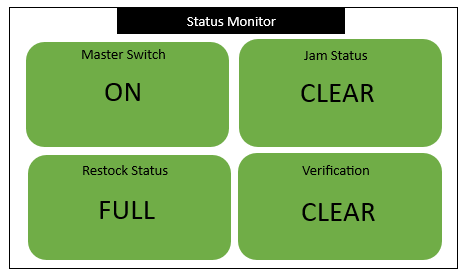
\includegraphics{statusgood.png}
    \caption{User Interface when system is functioning normally}
    \label{fig:scope}
  \end{figure}

  \begin{figure}[H]
    \centering
    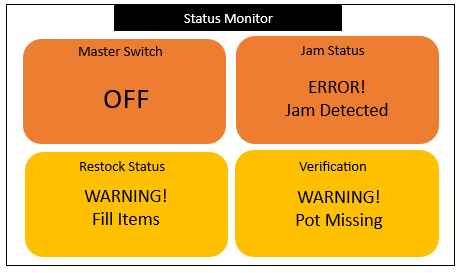
\includegraphics{statusbad.png}
    \caption{User Interface when errors arise}
    \label{fig:scope}
  \end{figure}
The user interface includes a screen with the output functions of the machine. The user does not have to interact with this device, as it is only used to provide information on the status of the Pot-pulator.
\subsection{Master Switch Status}
This section informs the user if the machine is on or off.
\subsection{Restock Status}
This section informs the user that the tray or pot dispenser is empty. The user will need to refill the pot dropper and the tray dispenser every 15 minutes.
\subsection{Verification}
This section informs the user if there is a pot missing or out of place once the trays reach the verification system.
\subsection{Jam Status}
This section informs the user that there is a jam in the stack of trays in the tray dispenser, or the stack of pots in the pot dropper. This will require the machine to be turned off and the trays and pots to be taken out and restacked. 
\newpage
\section{Features and Functionality}
\subsection{Conveyer}
To start the Pot-pulator, the user needs to press two switches located on the conveyer belt. Properly using these switches is crucial for the smooth operation of the machine. First, the black power switch should be pressed down to the line, then the red switch should be pressed down to the two lines. This ensures that the machine is ready to start and will function as needed.
\\
\noindent Once the switches have been set correctly, the conveyer belt will begin to move the trays through each system in the Pot-pulator. The conveyer will start and stop at specific positions to ensure that each tray is correctly positioned for pot dropping. This ensures that the system operates smoothly and that the pots are accurately placed in each tray.
\\
\noindent It's important to note that the conveyer belt must be properly maintained to ensure its longevity and proper functioning. Users should regularly clean it to remove any dirt, debris, or other materials that may accumulate on the belt. Additionally, users should inspect the conveyer belt regularly to ensure that it is functioning correctly.

\begin{figure}[H]
    \centering
    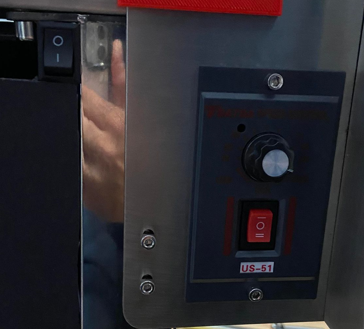
\includegraphics{switches.png}
    \caption{Both black and red switches should be switched down for proper function. This figure shows the Pot-Pulator powered off.}
    \label{fig:scope}
  \end{figure}
\newpage
\subsection{Tray Dispenser}
When using the tray dispenser system, it's important to note that up to 30 trays can be manually inserted into the top of the machine at the beginning of each refill. This allows for a continuous flow of trays, ensuring that there will be enough available for continuous use.
\\
\noindent The tray dispenser will need to be refilled every 15 minutes. This ensures that the machine doesn't run out of trays, which can cause delays and decrease the overall time efficiency of the device.
\\
\noindent To ensure proper functionality, it's recommended that the trays be stacked and placed evenly into the machine. This not only helps with the flow of trays through the dispenser, but also prevents jams and other issues that can arise from uneven stacking.
\\
\noindent By following these guidelines, users can ensure smooth and efficient tray dispensing, minimizing any downtime caused by errors.

\begin{figure}[H]
    \centering
    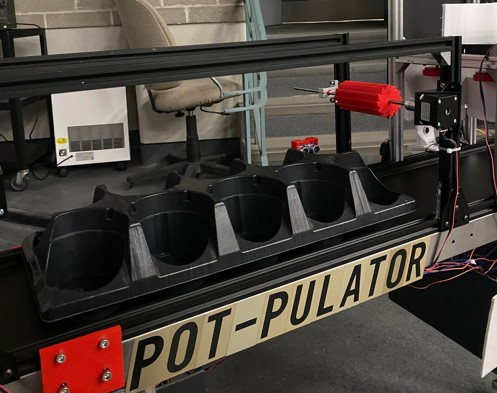
\includegraphics[width=0.8\textwidth]{tray.jpg}
    \caption{Tray Dispenser}
    \label{fig:scope}
  \end{figure}
\newpage
\subsection{Pot Dropper}
When using pot dropper system, the user can insert up to 300 pots manually into the uppermost section of the machine. Every 15 minutes, it is required for the user to refill the pot dropper to guarantee smooth operation of the device.
\\
\noindent It is important to note that the pot dropper contains two sections, each of which can accommodate a certain number of pots. To optimize the efficiency of the machine and guarantee an even distribution of pots, it is recommended that users stack and place pots in both sections uniformly. Proper stacking and placement of pots into the machine helps to prevent any issues such as jamming, or other operational malfunctions.
\\
\noindent By adhering to these guidelines, users can expect a reliable, efficient, and uninterrupted experience while using the pot dropper.

\begin{figure}[H]
    \centering
    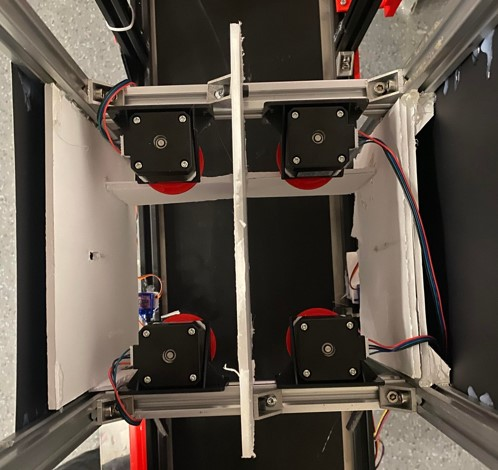
\includegraphics[width=0.8\textwidth]{pot.jpg}
    \caption{Pot Dropper}
    \label{fig:scope}
  \end{figure}
\newpage
\subsection{Verification System}
The verification system will notify the user when there is a problem with the system. If there is a pot missing or out of place, an LED will light up, alerting the user that the system is not functioning as intended. 
\section{Troubleshooting and FAQs}
\subsection{What happens if trays get stuck?}
If the trays get stuck, turn off the machine and remove them from the stack, and refill them evenly. Once they are in place, turn the machine on to run as normal.
\subsection{What happens if pots get stuck?}
If the pots get stuck, turn off the machine and remove them from the stack, and refill them evenly into both sections of the pot dropper. Once they are in place, turn the machine on to run as normal.
\subsection{How many trays can the tray dropper hold?}
The tray dropper can hold up to 30 trays, but it will need to be refilled every 15 minutes.
\subsection{How many pots can the pot dropper hold?}
The pot dropper can hold up to 300 pots, but it will need to be refilled every 15 minutes.
\subsection{How will I know that all the pots have been placed correctly in the tray?}
The verification subsystem will determine if all the pots have been placed correctly in the tray, outputting an LED and an error on the user interface when a pot is missing or out of place.
\subsection{How do I refill the Pot-pulator with trays and pots?}
When refilling pots and trays, ensure that the machine is turned off. 30 Trays and 300 pots can then be loaded evenly into their respective sections, the user can then turn on the machine for operation. The pot dropper has two sections, and the user can distribute them evenly between them.
\subsection{How do I use the user interface of the Pot-pulator?}
The user interface will display the current status of the machine. To learn more about the user interface and how to navigate it, please refer to the "User Interface" section of the manual.

\end{document}